\subsection{\texorpdfstring{\nitrogen{}}{15N} sensitivity-enhanced HSQC}
\label{subsec:noah__sehsqc_n}

I now move on to the \nitrogen{} seHSQC experiment, which (for small molecules) is an improvement on the HMQC experiment for two reasons: firstly, the PEP transfer grants additional sensitivity (and can be optimised for \ch{NH} groups); and secondly, splittings due to $\nJ{HH}$ are not observed in the indirect dimension.

Unsurprisingly, much of the discussion in the HMQC section is also relevant here.
For example, although both seHSQC modules already use two-gradient schemes and therefore do adequately suppress wing artefacts in later modules, the CTP gradient duration must still be lengthened in order to suppress bulk artefacts in the seHSQC itself.

\subsubsection{Sensitivity analysis}

To quantify these sensitivity gains, I ran several \noah{X,Sp,Cc} experiments, where the first module was a \nitrogen{} HSQC, seHSQC1, or seHSQC2 module (\cref{fig:n15_sens}).
Including the HSQC module in this analysis allows us to determine how much of the sensitivity gain is due to multiplet collapse, and how much is due to the sensitivity enhancement.
The value of both delays $\Delta$ and $\Delta'$ were set to $1 / (4 \cdot \oneJ{NH})$; no multiplicity editing was used.
The peak at \qty{8.0}{\ppm} is folded and is therefore omitted from this analysis.

\begin{figure}[!ht]
    \centering
    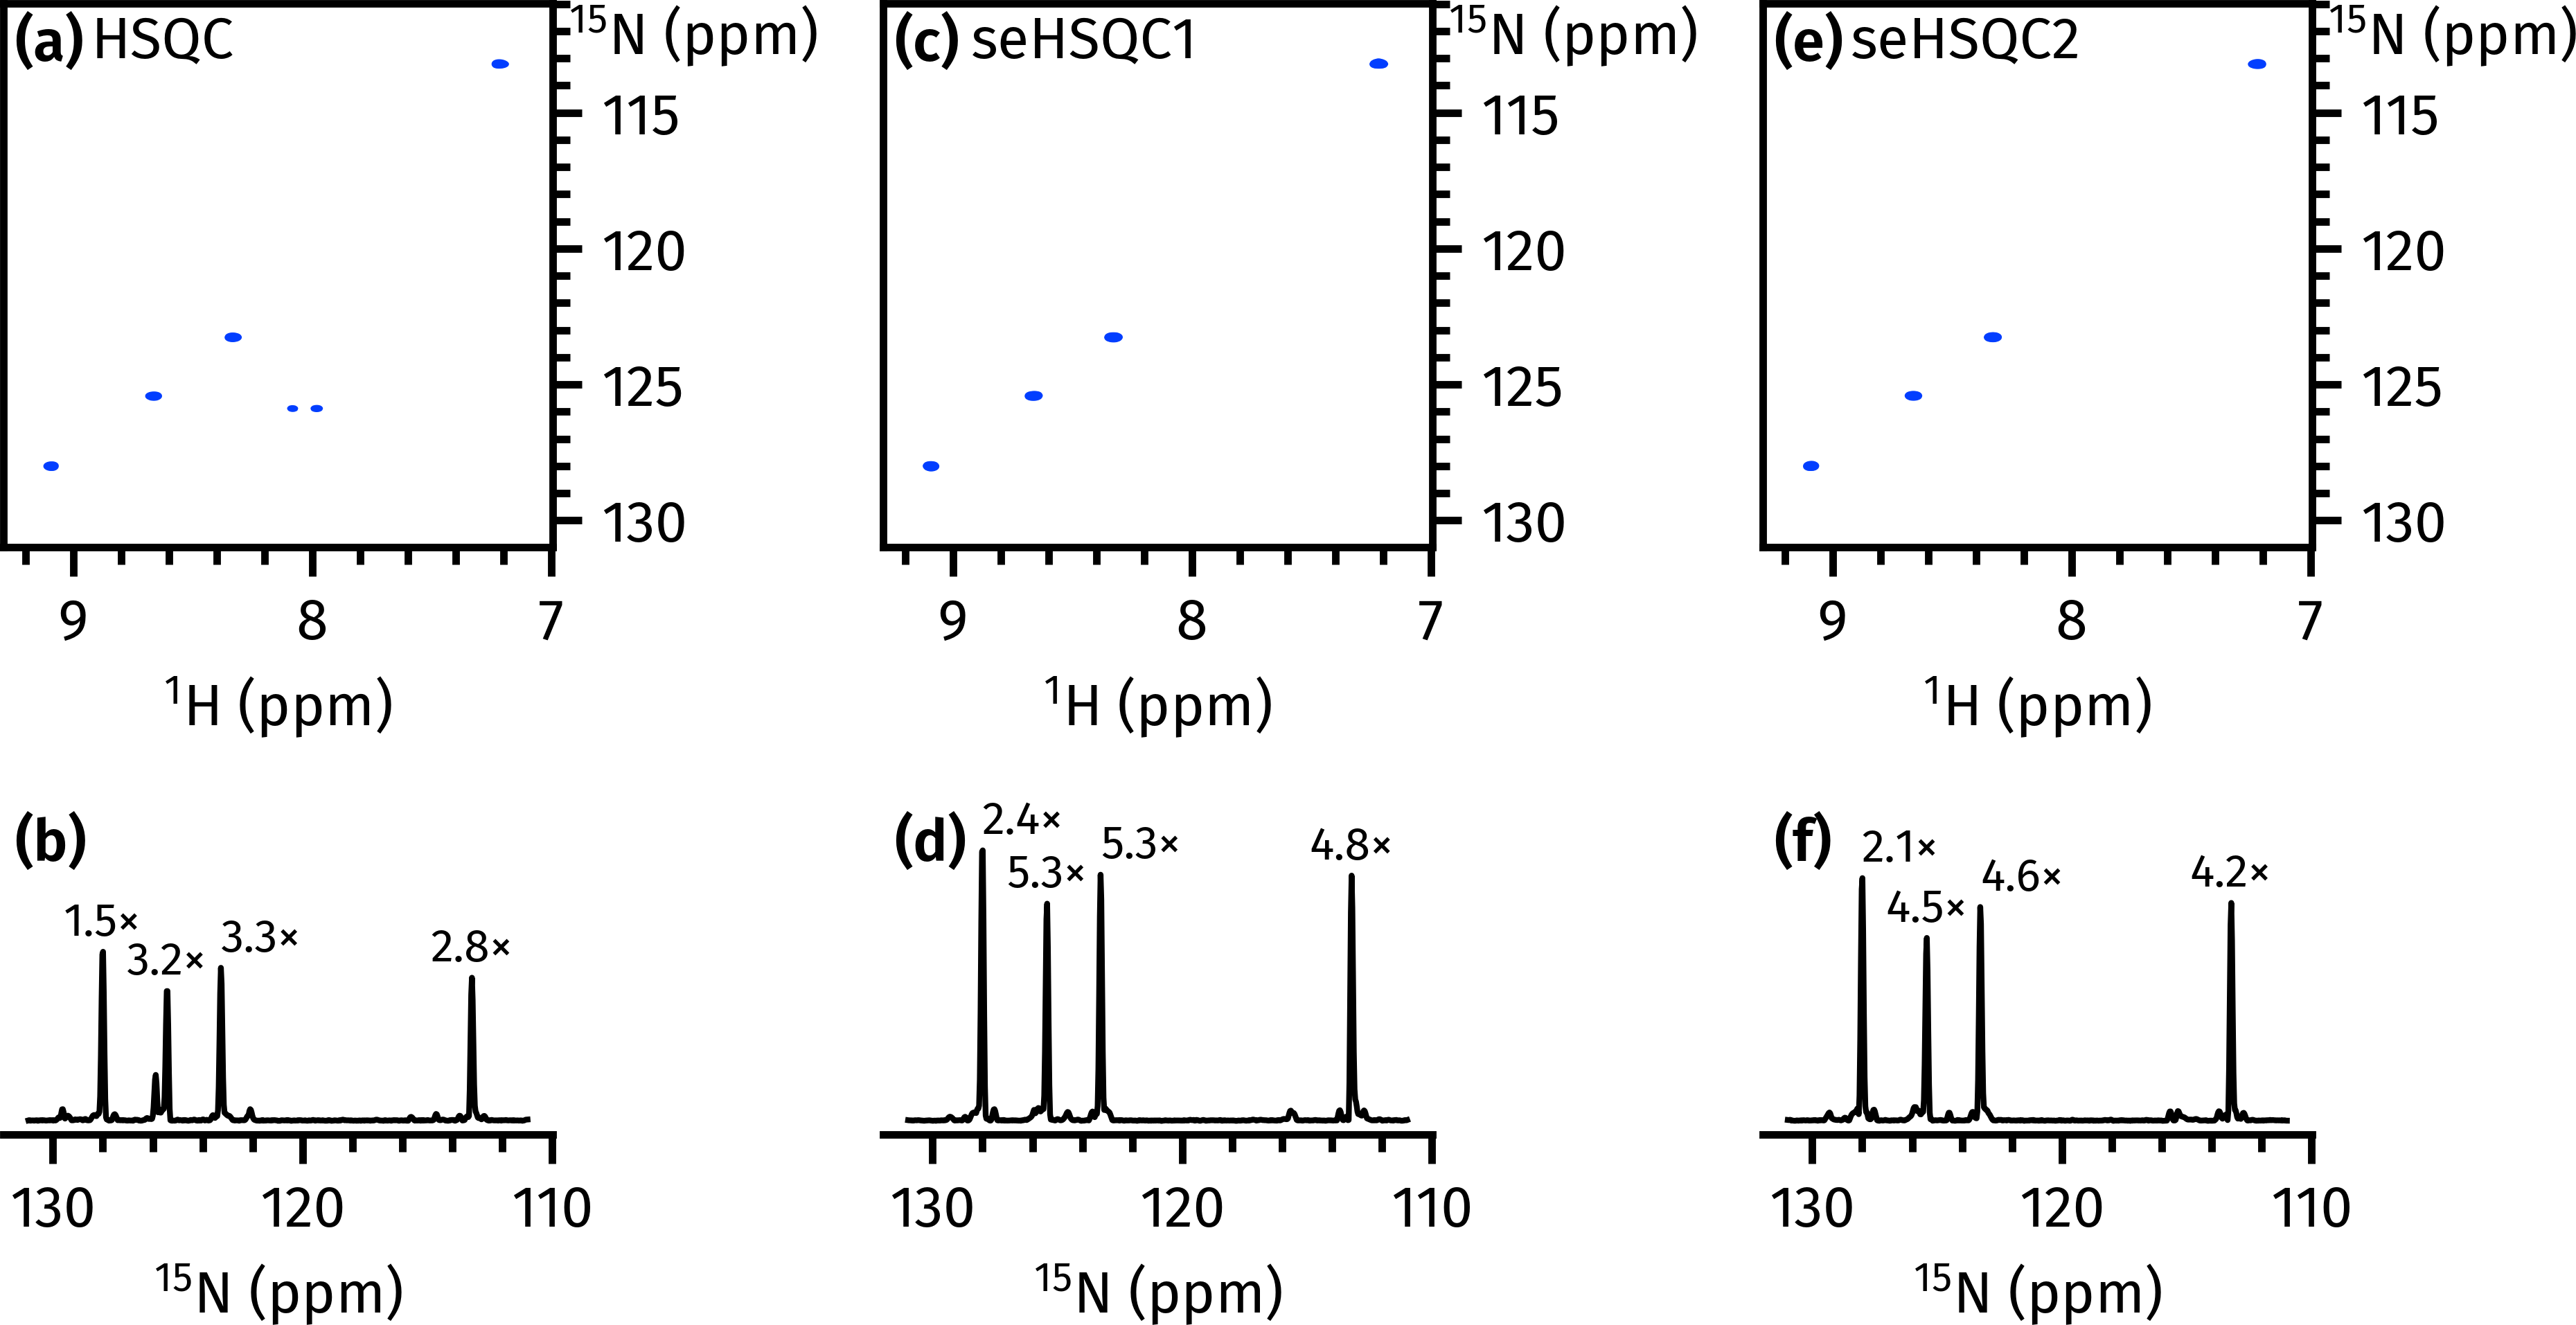
\includegraphics[draft=false]{noah/n15_modules_sens.png}%
    {\phantomsubcaption\label{fig:n15_sens_hsqc}}%
    {\phantomsubcaption\label{fig:n15_sens_hsqcp}}%
    {\phantomsubcaption\label{fig:n15_sens_sehsqc1}}%
    {\phantomsubcaption\label{fig:n15_sens_sehsqc1p}}%
    {\phantomsubcaption\label{fig:n15_sens_sehsqc2}}%
    {\phantomsubcaption\label{fig:n15_sens_sehsqc2p}}%
    \caption[Comparison of sensitivities of NOAH \nitrogen{} modules]{
        Comparison of NOAH \proton{}--\nitrogen{} modules; the 2D spectra and their positive projections onto the $F_1$ axis are shown.
        Numbers above each peak in the projections indicate sensitivity increases compared to the HMQC module (see, e.g., \cref{fig:hmqc_scale_std2,fig:hmqc_scale_std1}).
        \textbf{(\subref*{fig:n15_sens_hsqc})--(\subref*{fig:n15_sens_hsqcp})} HSQC module.
        \textbf{(\subref*{fig:n15_sens_sehsqc1})--(\subref*{fig:n15_sens_sehsqc1p})} seHSQC1 module.
        \textbf{(\subref*{fig:n15_sens_sehsqc2})--(\subref*{fig:n15_sens_sehsqc2p})} seHSQC2 module.
    }
    \label{fig:n15_sens}
\end{figure}

As can be seen, the HSQC alone allows for substantial sensitivity increases over the HMQC with over $3\times$ gains being accomplished simply due to multiplet collapse.
The seHSQC experiments push this even further, with an approximate $1.5\times$ sensitivity improvement for all peaks.
In contrast to the \carbon{} case, the \nitrogen{} seHSQC1 module outperforms seHSQC2 in terms of raw sensitivity, though (as before) there is no clear explanation for this subtle difference.

\todo{Compare other modules}


\subsubsection{CTP gradient duration}



\subsubsection{$k$-Scaling and linear prediction}

